\documentclass{report}
\usepackage[T1]{fontenc} % Fontes T1
\usepackage[utf8]{inputenc} % Input UTF8
\usepackage[backend=biber, style=ieee]{biblatex} % para usar bibliografia
\usepackage{csquotes}
\usepackage[portuguese]{babel} %Usar língua portuguesa
\usepackage{blindtext} % Gerar texto automaticamente
\usepackage[printonlyused]{acronym}
\usepackage{hyperref} % para autoref

\usepackage{}\usepackage{graphicx}

\bibliography{bibliografia}


\begin{document}
%%
% Definições
%
\def\titulo{Trabalho de aprofundamento}
\def\data{23-04-2018}
\def\autores{João Gameiro, Pedro Pereira}
\def\autorescontactos{(93097) joao.gameiro@ua.pt, (93196) pedrocjdpereira@ua.pt}
\def\versao{VERSAO}
\def\departamento{DETI}
\def\empresa{UA}
\def\logotipo{ua.pdf}
%
%%%%%% CAPA %%%%%%
%
\begin{titlepage}

\begin{center}
%
\vspace*{50mm}
%
{\Huge \titulo}\\ 
%
\vspace{10mm}
%
{\Large \empresa}\\
%
\vspace{10mm}
%
{\LARGE \autores}\\ 
%
\vspace{30mm}
%
\begin{figure}[h]
\center
\includegraphics{\logotipo}
\end{figure}
%
\vspace{30mm}
\end{center}
%
\begin{flushright}
\versao
\end{flushright}
\end{titlepage}

%%  Página de Título %%
\title{%
{\Huge\textbf{\titulo}}\\
{\Large \departamento\\ \empresa}
}
%
\author{%
    \autores \\
    \autorescontactos
}
%
\date{\data}
%
\maketitle

\pagenumbering{roman}

%%%%%% RESUMO %%%%%%
\begin{abstract}
Este relatório tem como objetivo a descrição e apresentação dos resultados do código desenvolvido no âmbito do projeto \ac{ap2} da disciplina de \ac{labi} do curso \ac{miect}.

De maneira a que um cliente possa verificar se a velocidade da sua internet corresponde à velocidade estabelecida previamente em contrato, existe uma rede de servidores, em que é possível avaliar a qualidade da ligação. 
O objetivo deste trabalho era criar um cliente para esses servidores, para que posteriormente pudesse ser feita uma avaliação da velocidade da internet.

Assim sendo, serão apresentados todos os recursos usados neste trabalho, desde biografias até módulos importados no código. O código desenvolvido será interpretado, tal como os seus resultados e é esperado que no fim da leitura deste relatório todo o código e resultados do mesmo sejam mais claros.

Quanto ao seu conteúdo, este relatório começa por descrever o código de programa, desde o modo como verifica os argumentos de entrada, ao estabelecimento de coneção com o servidor, passa depois pelo maneira como são efetuados os cálculos da latência e largura de banda e como os seus resultados são escritos num ficheiro csv. De seguida são efetuados testes para provar o funcionamento do código. Quando são inseridos erros propositados o programa reage corretamente, terminado e apresentando a mensagem de erro apropriada e, na ausência de erros, o programa funciona sem problemas e o ficheiro csv apresenta toda a informação correta. Para acabar o trabalho apresentam-se conclusões sobre o mesmo.

\end{abstract}




\tableofcontents
% \listoftables     % descomentar se necessário
% \listoffigures    % descomentar se necessário


%%%%%%%%%%%%%%%%%%%%%%%%%%%%%%%
\clearpage
\pagenumbering{arabic}

%%%%%%%%%%%%%%%%%%%%%%%%%%%%%%%%
\chapter{Introdução}
\label{chap.introducao}


O objetivo do programa é criar um cliente para servidores que servem para avaliação da velocidade da internet e a qualidade da ligação, permitindo ao cliente verificar se as capacidades da sua internet correspondem às estabelecidas previamente em contrato.

Este documento está dividido em quatro capítulos.
Depois desta introdução,
no \autoref{chap.metodologia} é apresentada a metodologia seguida na elaboração do código.
No \autoref{chap.resultados} são apresentados os resultados obtidos através de testes efetuados no programa,
e estes mesmos resultados são discutidos e analisados. 
Finalmente, no \autoref{chap.conclusao} são apresentadas
as conclusões do trabalho.

\chapter{Metodologia}
\label{chap.metodologia}

Neste capítulo será descrito todo o código desenvolvido, indicando 
e explicando a funcionalidade que o mesmo implementa e a maneira como a mesma foi implementada.

\section{Módulos Importados}

\begin{table}[htp]
\caption{Tabela Módulos Importados e as suas respetivas utilidades}
\end{table}%

\begin{tabular}{|l||c|} % Alinhamento: Esq, Centro, Dir
%
\hline
\large \textbf{Módulo} & {\large \textbf{Utilidade}} \\ \hline
sys &  Possibilita a passagem de argumentos ao programa \\ \hline
time & Determinação do tempo atual e para paragem do mesmo \\ \hline
datetime & Determinar a data atual \\ \hline
json & Abertura do ficheiro servers.json  \\ \hline
csv & Escrita de dados num ficheiro .csv  \\ \hline
socket & Para permitir a comunicação com o servidor \\ \hline
random & Calcular um valor aleatório \\ \hline
RSA & Para síntese de uma chave privada \\ \hline
\texttt{PKCS1\_OAEP} & útil na sínteses do ficheiro report.sig \\ \hline
%
\end{tabular}



\section{Condições iniciais}

\subsection{Argumentos de entrada}

Foi criado um if, para que se o número dos argumentos de entrada for menor que 3, o programa irá imprimir uma mensagem de erro a indicar esse acontecimento e posteriormente outra mensagem a referir o método de utilização (Ex.: {\itshape Usage method: python3 client.py interval num [country or id]} ).

Seguidamente fez-se uso do módulo sys para terminar o programa caso o número de argumentos não correspondesse ao pretendido.


\subsection{Intervalo e Número de Testes a Realizar}

Estas duas condições vão ser verificadas da mesma maneira.

Através do módulo sys vão ser lidos respectivamente o intervalo entre dois testes e o número de testes a serem realizados.

Sendo que são lidos dentro da instrução try, se ocorrer algum erro, a posterior instrução except irá "apanhá-lo" e imprimir uma mensagem de erro. Dentro do try foi também implementado um if em que se o valor inserido for menor ou igual a zero o programa irá terminar.

Nos dois caso foi usada a mesma metedologia.

\subsection{País ou id}

\begin{figure}[h]
\center % Centra as imagens
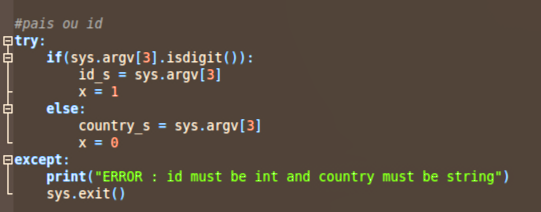
\includegraphics[height=100pt]{code.png}
\caption{Código para testar o argumento de entrada nº3}
\label{fig:code}
\end{figure}

Para o terceiro argumento foi novamente utilizado um try e dentro do mesmo testa-se se o argumento de entrada é composto por números ou letras. Dependendo do resultado é criada uma variável de estado para posterior utilização e se for por números considera-se como sendo o id ({\itshape \texttt{id\_s}}), por letras como sendo o país para o qual deve ser realizado o teste ({\itshape \texttt{country\_s}}). 

Se ocorrer algum o erro o programa imprime uma mensagem a indicar o mesmo e termina.

\subsection{Host}

Para a obtenção do Host foi necessário a abertura e leitura do ficheiro servers.json, o que foi feito com a ajuda do módulo json.


\subsubsection{ID}
Com a variável de estado x criada anteriormente, foi possível agora obter o host a partir do {\itshape \texttt{id\_s}} ou do {\itshape \texttt{country\_s}}. 
Logo se x tomar o valor de 1, é criado um for que percorre todos os ids pertencentes ao ficheiro servers.json e quando encontrar o correspondente para. Depois esse valor é guardado na variável {\itshape \texttt{final\_id}} para escrita no ficheiro report.csv e o host correspondente a esse id é obtido e guardado também em variáveis (utilização do método split) para fazer a ligação ao servidor. 

\subsubsection{Country}
Se x tomar o valor 0, os países presentes no ficheiro json vão ser corridos e quando se encontrar o correspondente ao inserido no argumento é adicionado a uma lista l o seu respetivo host. Adicionalmente é criada outra lista i para armazenar os ids. 
Após isto faz-se uso do módulo random para escolher da lista um host para usar na conexão ao servidor. É também criado um ciclo for para percorrer todos os hosts e obter a posição do host escolhido que depois será usada para alcançar o valor de {\itshape \texttt{final\_id}}. 


\begin{figure}[h]
\center % Centra as imagens
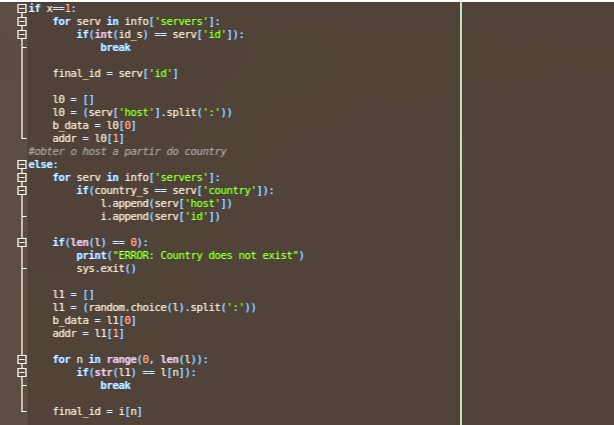
\includegraphics[height=240pt]{code0.png}
\caption{Código para obtenção do host}
\label{fig:code0}
\end{figure}


Após tudo isto, com apoio do módulo csv é aberto o ficheiro report.csv para a escrita dos dados que vão ser obtidos.



\section{Comunicação com o servidor}

Toda a comunicação com o servidor é feita dentro de um ciclo for que se repete n vezes (sendo o n o número de testes inserido como argumento).


Para a comunicação com o servidor vão ser usadas 4 Strings:
\begin{description}
\item[HI] - que vai receber a resposta HELLO com identificação do software;
\item[PING] - acompanhado com time.time()que corresponde ao tempo em microsegundos que irá receber a resposta PONG;
\item[DOWNLOAD] - acompanhado pela quantidade em octetos que o utilizador quiser.
\item[QUIT] - para terminar o programa
\end{description}

Assim sendo, dentro de um try é feita a conexão ao servidor criando-se
um socket que terá como argumentos {\itshape \texttt{b\_data}} e {\itshape \texttt{addr}} obtidos anteriormente. Se a ligação for bem sucedida então é apresentada uma mensagem a prová-lo e é registado o tempo. Caso contrário é apresentada uma mensagem de erro e a largura e a latência tomam valores 0 e -1 respectivamente pois estão na presença de uma conexão falhada.

\begin{figure}[h]
\center % Centra as imagens
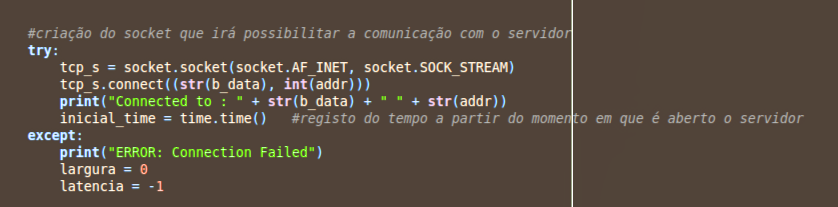
\includegraphics[height=90pt]{code1.png}
\caption{Ligação ao servidor}
\label{fig:code1}
\end{figure}

\subsection{HI}
 Das strings criadas anteriormente é enviada ao servido a string HI.
 Em seguida é criada uma variável {\itshape \texttt{resulthello}} que vai receber a resposta do servidor e que será impressa (será a identificação do software).
 
 
\begin{figure}[h]
\center % Centra as imagens
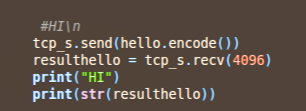
\includegraphics[height=65pt]{code2.png}
\caption{Comando HI}
\label{fig:code2}
\end{figure}

\subsection{PING}

Antes do envio do comando PING para o servidor é criada uma lista que irá armazenar o valor devolvido pelo PONG. 

Como em cada teste ocorrem 10 interacções PING/PONG, foi criado um ciclo for que irá repetir-se 10 vezes.

Dentro de cada ciclo é em primeiro lugar enviado para o servidor o comando PING acompanhado com o tempo atual em microsegundos, em segundo lugar é armazenada a resposta devolvida (PONG + tempo do servidor) numa variável. Essa variável é dividida (método split) em PONG e tempo do servidor. Da divisão retiramos o tempo do servidor e adiciona-mo-lo à lista criada anteriormente.

Após todos os 10 ciclos completos é impresso no ecrã o conteúdo da lista com o número à frente que serve como contagem do número de PONGS recebidos (o último tem de ser sempre 10).


\begin{figure}[h]
\center % Centra as imagens
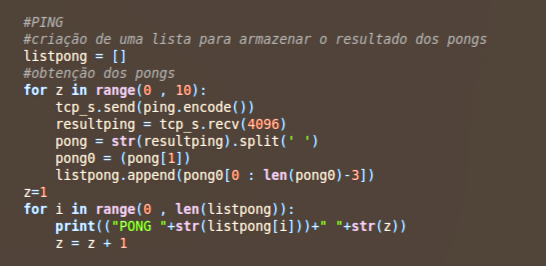
\includegraphics[height=130pt]{code4.png}
\caption{Comando PING}
\label{fig:code4}
\end{figure}



\subsection{DOWNLOAD}

Antes da início do download é registado o tempo, que servirá para verificar se já passaram 10 segundos ou não. Por isso todo o processo de troca de informação envolvendo o DOWNLOAD é realizado dentro de um if que certifica que o DOWNLOAD tem de ser feito até que passem 10 segundos.

É iniciada uma variável {\itshape \texttt{numd}} que é recebida pelo teclado e que tem de pertencer ao intervalo [10, 100] (daí o assert presente na linha seguinte). 

Após isso é registado o tempo antes do início do download e enviado para o servidor o valor inserido através do comando DOWNLOAD. A seguir à recepção da resposta do servidor regista-se o tempo (irá ser usado para calcular a largura de banda) e imprime-se a informação recebida.


\begin{figure}[h]
\center % Centra as imagens
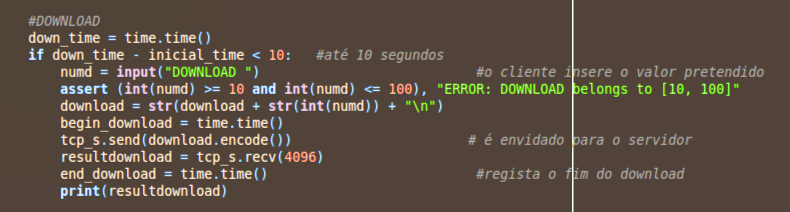
\includegraphics[height=90pt]{code5.png}
\caption{Comando DOWNLOAD}
\label{fig:code5}
\end{figure}



 \subsection{QUIT}
 Após termos todos os dados necessários para o objetivo pretendo, é enviado ao servidor o comando QUIT o que irá fechar a ligação com o mesmo. É fechado também o socket com o comando {\itshape \texttt{tcp\_s.close()}}.
 
\begin{figure}[h]
\center % Centra as imagens
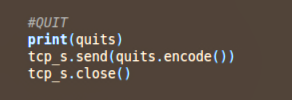
\includegraphics[height=60pt]{code3.png}
\caption{Comando QUIT}
\label{fig:code3}
\end{figure}

\section{Latência e Largura}

\begin{itemize}
\item \textbf{Latência};
\end{itemize}

Ao calcular a média dos valores retornados pelos PONGS obtemos a latência. Por isso foi criada uma variável {\itshape \texttt{soma}} que corresponde à soma e todos os valores da lista que armazenava os PONGS, que foi dividida pelo número de elementos dessa lista.

O resultado foi imprimido no terminal.

\begin{itemize}
\item \textbf{Largura de Banda};
\end{itemize}
A Largura de Banda foi calculada ao ser dividido o valor do download por um delta tempo. Esse delta tempo corresponde ao tempo que o servidor demorou a enviar a quantidade indicada anteriormente e foi calculado com a ajuda dos valores de {\itshape \texttt{end\_download}} e {\itshape \texttt{begin\_download}}.

Tal como a latência, também o valor da largura foi posteriormente imprimido.


\begin{figure}[h]
\center % Centra as imagens
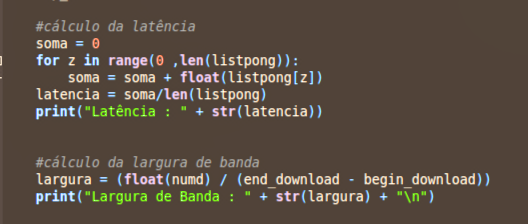
\includegraphics[height=110pt]{code6.png}
\caption{Cálculo da Latência e da Largura de Banda}
\label{fig:code6}
\end{figure}



\section{Escrita dos Resultados}
Os resultados obtidos, da latência e da largura de banda, tal como o id do servidor foram escritos num ficheiro report.csv.
    
Ficheiro esse que contém também a data actual (uso do módulo datetime), o número de testes e um campo check que contém todos os dados juntos sem qualquer tipo de separador.

De referir mais um facto, no fim da escrita dos dados, existe um trecho que para o tempo se houver mais algum teste a ser feito, de acordo com o valor especificado nos argumentos de entrada, ou seja é o intervalo de espera entre cada teste.

\section{Chave Privada}

Após todas as informações foi criada uma chave privada {\itshape \texttt{key}} e lido um ficheiro key.priv que continha síntese dessa chave. Foi também criado o report.sig que contém as mesmas informações que o report.csv e que tem a assinatura da chave privada.


\begin{figure}[h]
\center % Centra as imagens
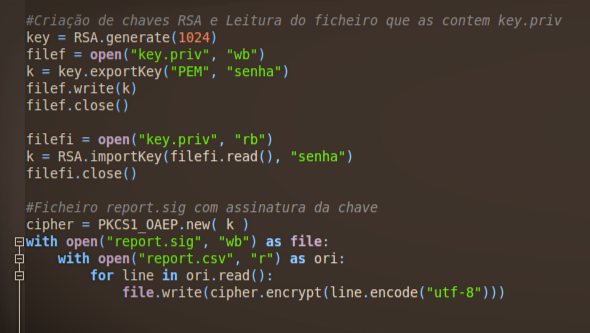
\includegraphics[height=140pt]{code7.png}
\caption{Chave privada e ficheiro report.sig}
\label{fig:code7}
\end{figure}





 \chapter{Resultados e Análise}
\label{chap.resultados}
Neste capítulo vão ser descritos os resultados obtidos pelo programa.
\section{Erros Iniciais Propositados}

\begin{figure}[h]
\center % Centra as imagens
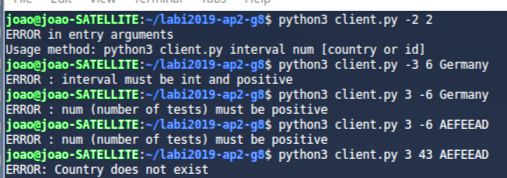
\includegraphics[height=90pt]{test.png}
\caption{Erros iniciais}
\label{fig:test}
\end{figure}

Como podemos ver na \autoref{fig:test}, se for iniciado com argumento inferior a 3 imprime uma mensagem de erro e termina, tal como se o intervalo e o número de testes for menor que 0. Se o país não existir também não inicia.

Se for indicado um id inválido, o programa vai por opção de default realizar os testes para o host {\itshape \texttt{speedtest.ushuaiavision.com.ar 8080}}

\section{Testes Funcionais com ID e com País}
 
 Ao realizarmos o teste para o id 21239 verificamos que corre tudo como o esperado(são realizados dois testes, 1 segundo de espera entre cada um e todas as funcionalidades descritas comportam-se como esperado)(\autoref{fig:test1}).
 
 Se realizarmos para um país constamos que também ocorre tudo como esperado.(\autoref{fig:test2})
 

 
\begin{figure}[h]
\center % Centra as imagens
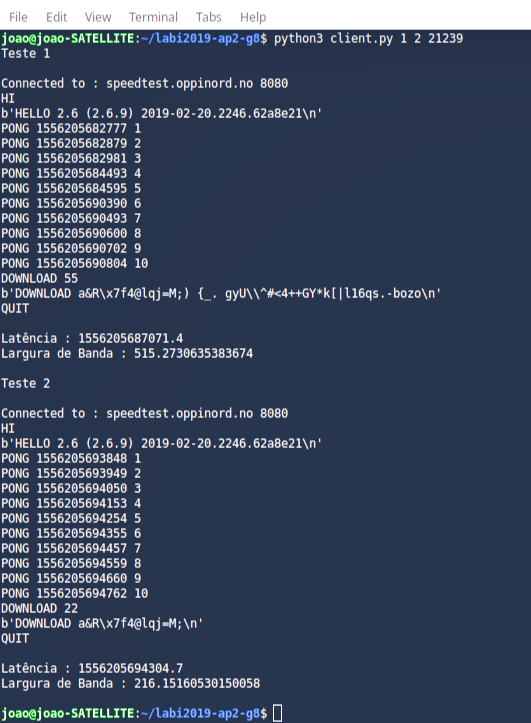
\includegraphics[height=300pt]{test1.png}
\caption{Teste Funcional ID}
\label{fig:test1}
\end{figure}

\begin{figure}[h]
\center % Centra as imagens
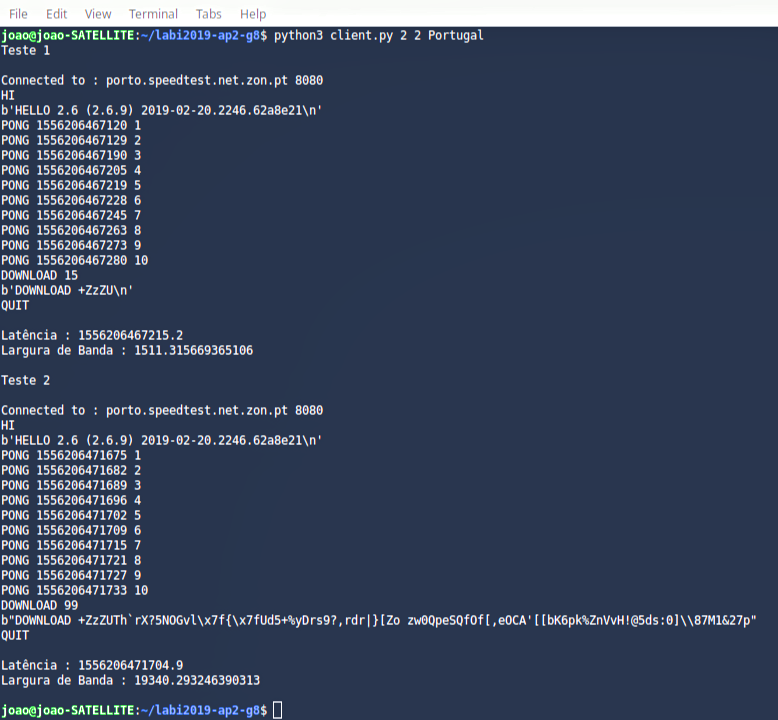
\includegraphics[height=300pt]{test2.png}
\caption{Teste Funcional País}
\label{fig:test2}
\end{figure}

O report.csv contém todas as informações especificadas nos testes e foi criada uma chave e um ficheiro report.sig.



\section{Erro DOWNLOAD}
Na \autoref{fig:test3} é possível verificar que se o valor do DOWNLOAD não pertencer a [10, 100] ocorre um erro.

\begin{figure}[h]
\center % Centra as imagens
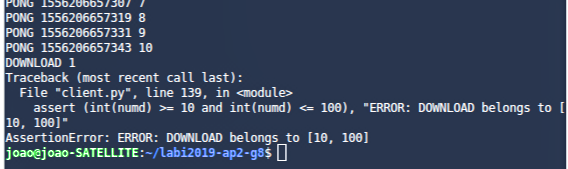
\includegraphics[height=100pt]{test3.png}
\caption{Erro Download}
\label{fig:test3}
\end{figure}


Na \autoref{fig:test4} também é possível ver a chave RSA e um ficheiro report.csv de um teste anteriormente realizado.

\begin{figure}[h]
\center % Centra as imagens
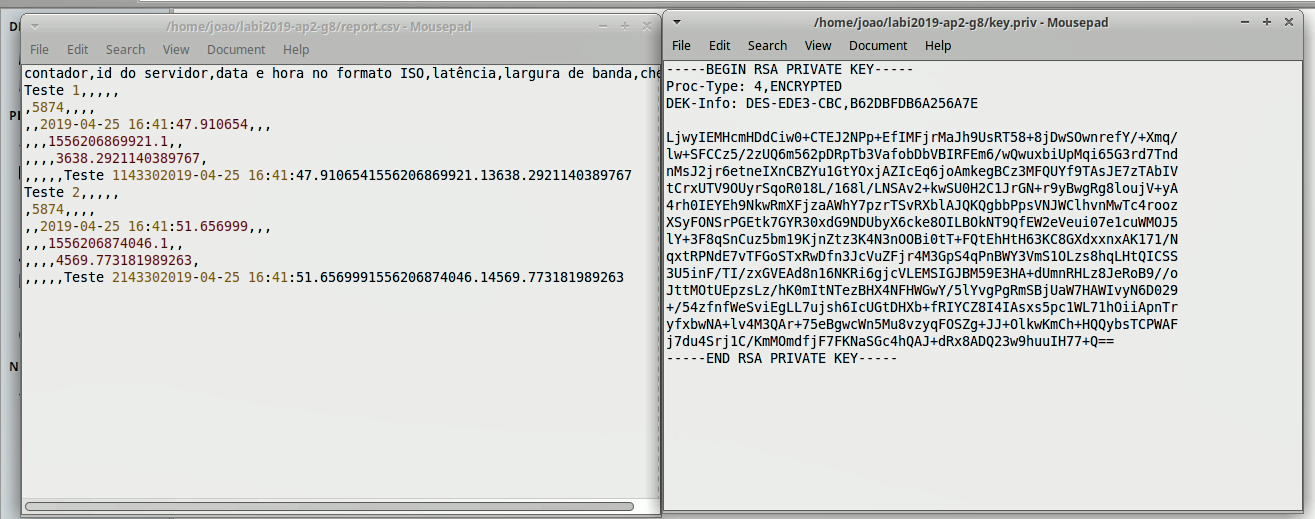
\includegraphics[height=150pt]{test4.png}
\caption{Chave RSA e report.csv}
\label{fig:test4}
\end{figure}


\chapter{Conclusões}
\label{chap.conclusao}
Com o trabalho concluído, é possível comprovar o correto funcionamento do programa criado, capaz de avaliar a velocidade da internet do cliente através da sua execução acompanhada por argumentos válidos. Compreendendo melhor o seu funcionamento entende-se, assim, a utilidade de uma aplicação como esta bem como a importância deste projeto para o desenvolvimento das capacidades de escrita de código em python dos seus autores.

\chapter*{Contribuições dos autores}
Todo o código foi discutido e desenvolvido em conjunto. A estrutura do relatório foi também discutida em conjunto, sendo  que \ac{jg} escreveu os capítulos \autoref{chap.metodologia} e \autoref{chap.resultados} e \ac{pp} escreveu os capítulos \autoref{chap.introducao} e \autoref{chap.conclusao}. Considera-se que cada autor contribuiu igualmente para este trabalho logo a atribuição de percentagens é \ac{jg} - 50\%  e \ac{pp} - 50\%.

\section{Code UA e ShareLatex}
Aqui encontra-se o link para o projeto usado na plataforma Code UA.
\begin{itemize}
\item {https://code.ua.pt/projects/labi2019-ap2-g8/repository};
\end{itemize}

Para o desenvolvimento do relatório como foi usada a plataforma ShareLatex, por isso não exite nenhuma versão do mesmo no Code UA.

\section{Nota Final}
\cite{labi}

 O código desenvolvido, conteúdo apresentado e estrutura do relatório tiveram como principal apoio os Guiões e PowerPoints da disciplina  \ac{labi} da \ac{ua} fornecidos aos alunos.


%%%%%%%%%%%%%%%%%%%%%%%%%%%%%%%%%
\chapter*{Acrónimos}
\begin{acronym}
\acro{ap2}[AP2]{Trabalho de Aprofundamento 2}
\acro{labi}[LABI]{Laboratórios de Informática}
\acro{ua}[UA]{Universidade de Aveiro}
\acro{miect}[MIECT]{Mestrado Integrado em Engenharia de Computadores e Telemática}
\acro{jg}[JG]{João Gameiro}
\acro{pp}[PP]{Pedro Pereira}
\end{acronym}


%%%%%%%%%%%%%%%%%%%%%%%%%%%%%%%%%
\printbibliography

\end{document}
